% base off spec, but adapt to new system
% have a brief description of func reqs (what they are)

The functional requirements describe the technical capabilities of the implemented aspect of the project.
They detail how the system should react in certain scenarios, and state what services the system should be able to provide.
The can also state limitations in the scope of the system, i.e. routes of development that are not intended to be implemented \cite{software_engineering_req_analysis}.

\begin{enumerate}[label=\textbf{F\arabic*:}]
  \item The system \textbf{must} allow the modelling of a network with at least three switches and four hosts, arranged in a tree topology as shown in figure \ref{minimum_tree}.
  \item The system \textbf{must} allow switches and hosts to be configured in a tree topology.
  \item The system \textbf{must} allow users to specify the spread of the network when using a tree topology (i.e. how many children a switch node will have).
  \item The system \textbf{must} allow users to specify the number of levels in the network when using a tree topology.
  \item The system \textbf{must} allow users to specify which level in the network should be modelled as FPGA-based smart network switches.
  \item The system \textbf{must} allow users to run a test to ensure there is an active connection between all hosts.
  \item The system \textbf{must} allow users to run a test to display the bandwidth of the system.
  \item The system \textbf{must} allow users to run a test to display the delay between the leaf nodes and the root when using a tree topology.
  \item The system \textbf{should} allow users to specify the bandwidth of all links in the network.
  \item The system \textbf{should} allow users to specify the delay of all links in the network.
  \item The system \textbf{should} allow users to specify the chance of packet loss for all links in the network.
  \item The system \textbf{should} allow switches and hosts to be configured in a vertical linear topology.
  \item The system \textbf{should} employ multiple levels of logging.
  \item The system \textbf{should} conform to \textit{Python}'s PEP8 code standard \cite{python_pep8}.
  \item The system \textbf{should} be made open-source.
  \item The system \textbf{could} allow users to configure the system to use a Poisson distribution for link delays.
  \item The system \textbf{could} allow users to configure the bandwidth of FPGA-based smart network switch nodes.
  \item The system \textbf{could} allow users to configure the delay of FPGA-based smart network switch nodes.
  \item The system \textbf{could} allow users to configure the chance of packet loss of FPGA-based smart network switch nodes.
  \item The system \textbf{could} allow users to display all node connections before running tests.
  \item The system \textbf{won't} be configured for IPv6 connections.
\end{enumerate}


\begin{figure}[t]
  \centering
  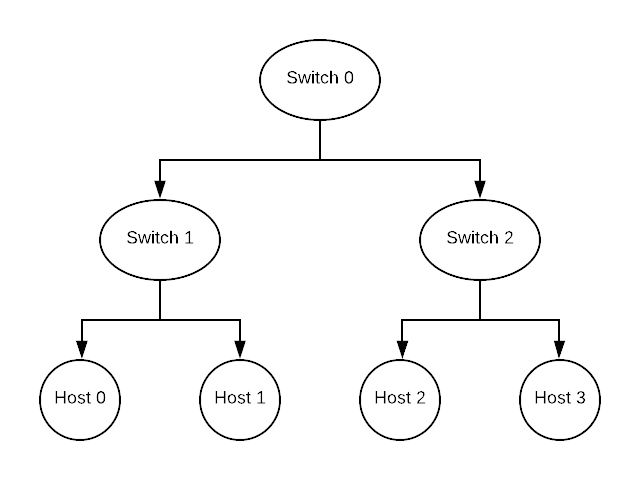
\includegraphics[width=\textwidth]{assets/minimum_tree.png}
  \caption{The required minimum tree topology}
  \label{minimum_tree}
\end{figure}

% \begin{enumerate}[label=\textbf{F\arabic*:}]
%   \item The system \textbf{must} be able to analyse packets at layer 2 of the OSI network model
%   \item The system \textbf{must} be able to send packets to the correct port based on MAC addresses
%   \item The system \textbf{must} be able to store MAC address tables
%   \item The system \textbf{must} be able to dynamically update MAC address tables
%   \item The average latency of the system \textbf{must} be measured
%   \item The throughput of the system \textbf{must} be measured
%   \item The system \textbf{should} be able to analyse packets at layer 3 of the OSI network model
%   \item The system \textbf{could} be able to analyse packets at layer 7 of the OSI network model
%   \item The system \textbf{could} be able to detect basic network attacks (such as TCP SYN Flooding \cite{rfc4987})
%   \item The system \textbf{could} implement features of a basic firewall (such as packet filtering \cite{rfc2979})
% \end{enumerate}
